\documentclass[tikz,border=8pt]{standalone}
% Shared look for every TikZ diagram. Load with \input{../../tools/tikz-style.tex}
\usepackage[T1]{fontenc}
\usepackage{lmodern}
\renewcommand{\sfdefault}{lmr}  % diagrams use the same serif as the text
\usetikzlibrary{arrows.meta, positioning, shapes.geometric, calc, fit, backgrounds}
\definecolor{cblue}{HTML}{4C78A8}
\definecolor{corange}{HTML}{F58518}
\definecolor{cgreen}{HTML}{54A24B}
\definecolor{cred}{HTML}{E45756}
\definecolor{cpurple}{HTML}{B279A2}
\definecolor{cgrey}{HTML}{6B6B6B}
\tikzset{
  every picture/.style={font=\sffamily, line width=1.2pt},
  box/.style={draw=#1, fill=#1!12, rounded corners=4pt, align=center, inner sep=7pt, minimum height=1.1cm},
  box/.default=cgrey,
  arrow/.style={-{Stealth[length=3mm]}, draw=cgrey, line width=1.4pt},
  title/.style={font=\sffamily\bfseries\Large},
  note/.style={font=\sffamily\small, text=cgrey, align=center},
}
\AtBeginDocument{\hyphenpenalty=10000 \exhyphenpenalty=10000}

% What the robot knows and what it does not. Top row: the true cells (hidden from the robot). Bottom rows: the
% commands it gave and the readings it got. The history grows by one command and one reading every step.
\definecolor{cbrown}{HTML}{9C755F}
\begin{document}
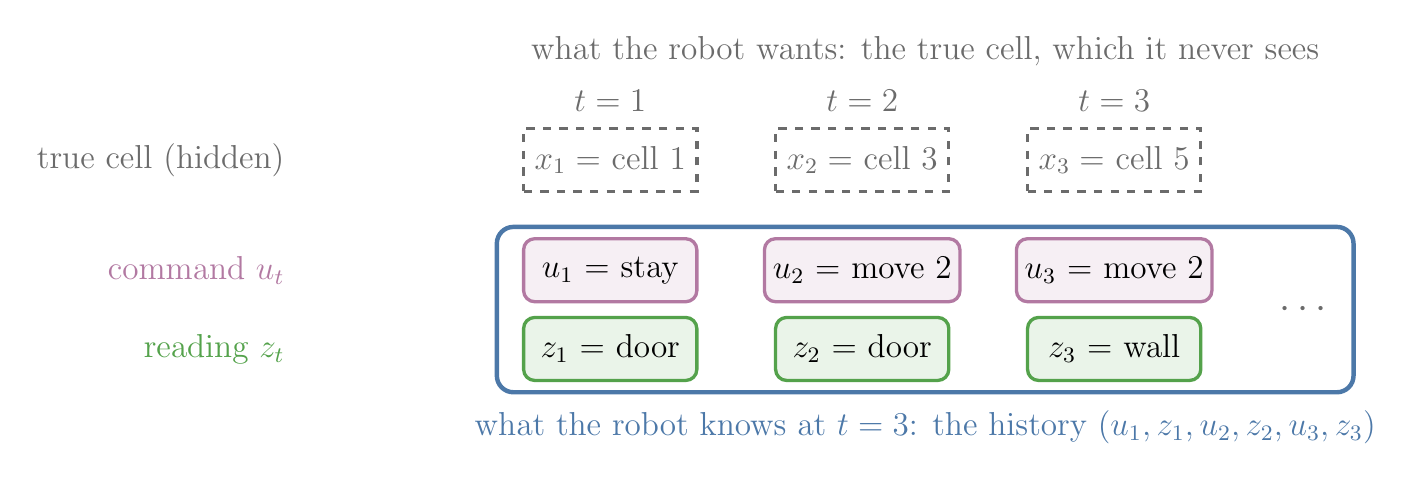
\begin{tikzpicture}[x=3.2cm, y=1cm, every node/.append style={font=\large}]
  \node[anchor=east, cgrey] at (-0.25,3) {true cell (hidden)};
  \node[anchor=east, cpurple] at (-0.25,1.6) {command $u_t$};
  \node[anchor=east, cgreen] at (-0.25,0.6) {reading $z_t$};
  \foreach \t/\x/\u/\z in {1/1/stay/door, 2/3/move 2/door, 3/5/move 2/wall} {
    \node[draw=cgrey, dashed, text=cgrey, minimum width=2.2cm, minimum height=0.8cm] at (\t,3) {$x_\t = $ cell \x};
    \node[box=cpurple, minimum width=2.2cm, minimum height=0.8cm, inner sep=3pt] at (\t,1.6) {$u_\t$ = \u};
    \node[box=cgreen, minimum width=2.2cm, minimum height=0.8cm, inner sep=3pt] at (\t,0.6) {$z_\t$ = \z};
    \node[cgrey] at (\t,3.75) {$t = \t$};
  }
  \node[cgrey, font=\Large] at (3.75,1.1) {$\cdots$};
  % what the robot knows
  \draw[cblue, line width=1.6pt, rounded corners=6pt] (0.55,0.05) rectangle (3.95,2.15);
  \node[cblue, anchor=north] at (2.25,-0.05) {what the robot knows at $t = 3$: the history $(u_1, z_1, u_2, z_2, u_3, z_3)$};
  \node[cgrey, anchor=south] at (2.25,4.05) {what the robot wants: the true cell, which it never sees};
\end{tikzpicture}
\end{document}
